\begin{figure}[h]
	\centering
	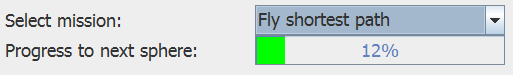
\includegraphics[width=0.6\textwidth]{AutopilotGUI.png}
	\caption{De \textit{GUI} van de Autopilot. Hierop is het dropdownmenu te zien waar de gewenste missie kan geselecteerd worden. Ook de vooruitgang naar de volgende (in dit geval groene bol) is waar te nemen.}
\end{figure}
\begin{figure}[h]
	\centering
	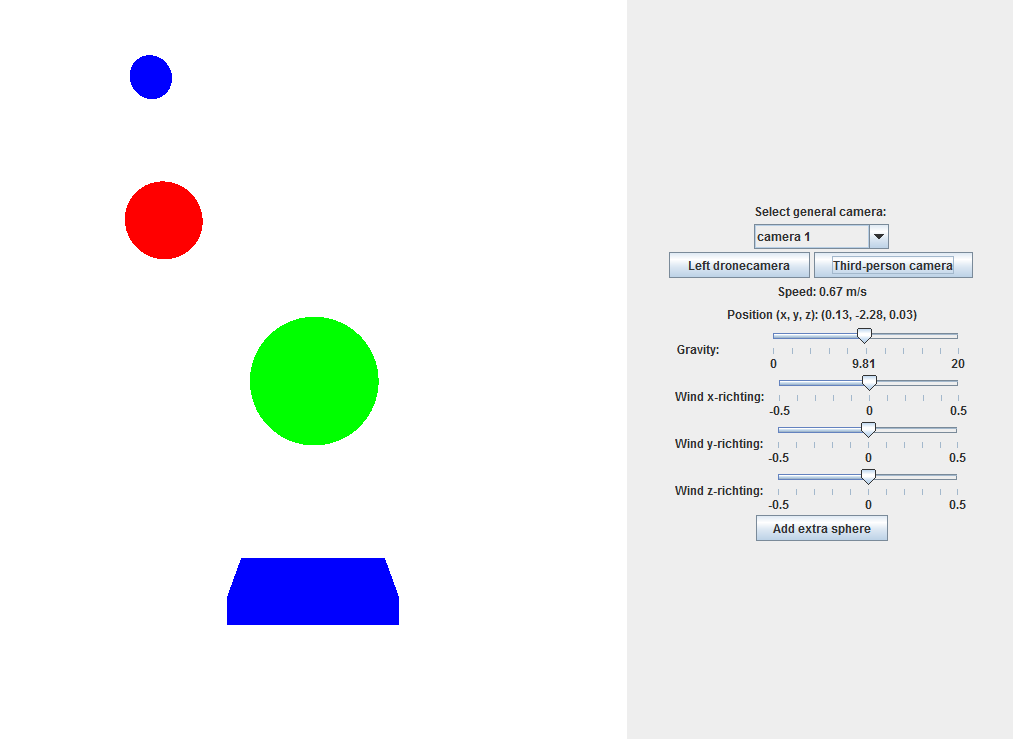
\includegraphics[width=0.9\textwidth]{TestbedGUI.png}
	\caption{De \textit{GUI} van het Testbed. De camera kan gekozen worden a.d.h.v. het dropdownmenu of de twee extra buttons. Daarnaast wordt de ogenblikkelijke snelheid en positie van de drone weergeven. Via de schuifbalken is het mogelijk de wind en gravitatieconstante aan te passen. Om uiteindelijk een extra bol (via co\"ordinaten) toe te voegen wordt de laatste button gebruikt. Zoals in sectie \ref{sec:GUIVirtualTestbed} aangehaald, veranderen de schuifbalken in sommige gevallen naar de weergave van ingestelde windsnelheden.}
\end{figure}